\chapter{Other Simulations}
\section{Effect of array tilt on ground reflections}\label{sec:refTilted}
\begin{figure}[!ht]
\centering
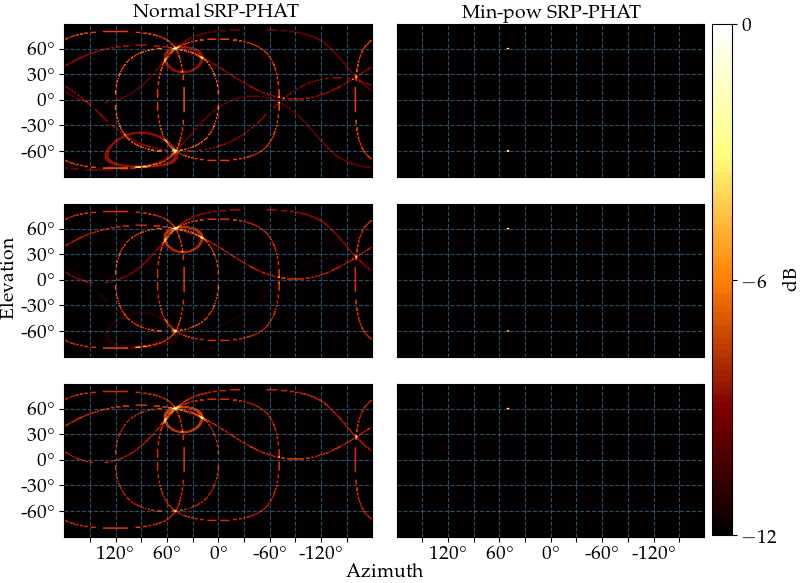
\includegraphics[width=\textwidth]{Figures/refSim.png}
\caption{Figures depict from top-to-bottom SRP-PHAT localization results with ground reflection coefficients (R) of 1, 0.6 and 0.1. The array has been tilted 30$\degree$ along the X-axis and 15$\degree$ along the Y-axis. This causes the ground image source to stop sharing cones with the real source and the correct relative power level between the image and real source is maintained for both normal SRP-PHAT and Min-pow SRP-PHAT}
\label{fig:4mic1srcRefTilt}
\end{figure}
Keeping the tetrahedral array horizontal\footnote{Such that three of its microphones are at the same height}, causes ground image source and the main source to share 3 out of 6 localization cones. This can cause magnitude errors when localizing with normal SRP-PHAT. This issue can be solved by tilting the microphone array as can be seen in Fig. \ref{fig:4mic1srcRefTilt}. As an effect of tilting the tetrahedron 30$\degree$ along the X-axis and 15$\degree$ along the Y-axis, the localization cones stop overlapping. 


\section{Effect of angular resolution of localization}\label{app:angRes}
Similar to the 2D angular resolution due to a single pair (Fig. \ref{fig:res_diff}), the tetrahedral array has its own 3D  angular resolution depending on the sample rate and the array aperture size. Fig. \ref{fig:res_diff_3d} describes the angular resolution of a tetrahedral array of aperture 1m for different sample rates. If the SRP search space is $360\degree$ by $180\degree$, and the resolution of search is $1\degree$, there will be some angular locations where the delay in sample between a microphone pair is fractional. For simplicity, this fractional delay is rounded for all plots in this thesis. This means that certain locations will contain duplicate data from the nearest integral delay location to themselves. Obviously, the resolution improves for higher sample rate.
\begin{figure}[H]
    \centering
    \begin{subfigure}[b]{0.96\textwidth}
    \centering
    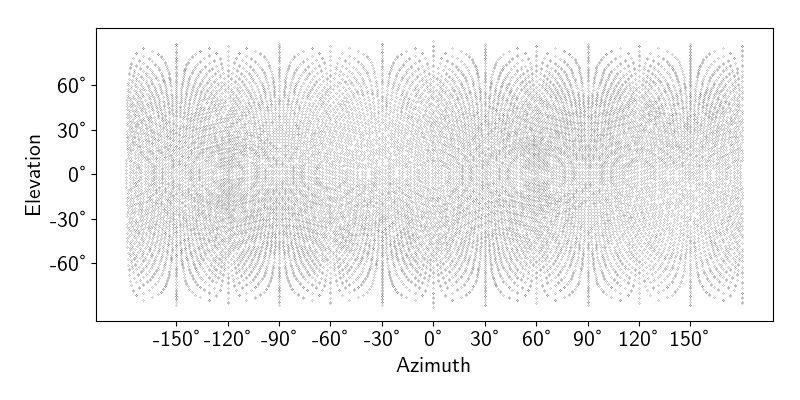
\includegraphics[width=0.7\textwidth]{Figures/res3d12k.png}
\end{subfigure}
\vskip \baselineskip
\begin{subfigure}[b]{0.96\textwidth}
    \centering
    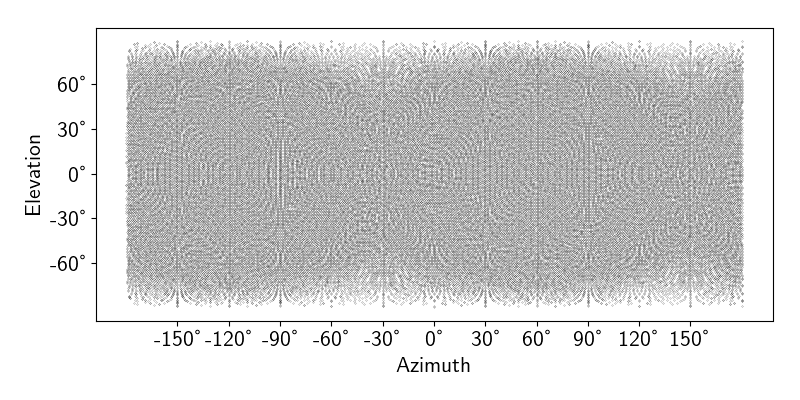
\includegraphics[width=0.7\textwidth]{Figures/res3d48k.png}
\end{subfigure}
\vskip \baselineskip
\begin{subfigure}[b]{0.96\textwidth}
    \centering
    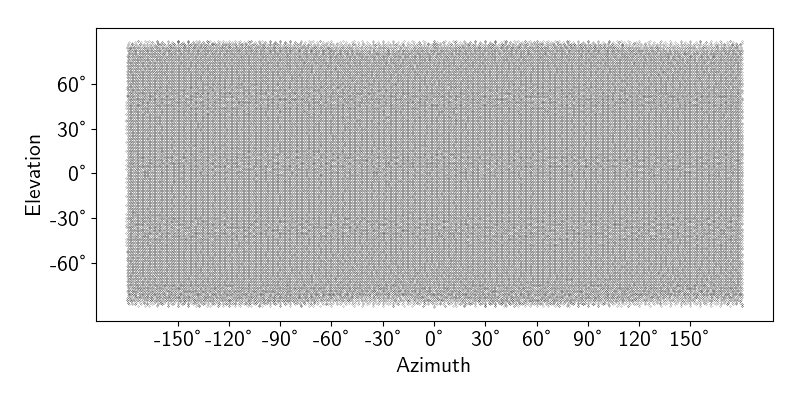
\includegraphics[width=0.7\textwidth]{Figures/res3d192k.png}
\end{subfigure}
    \caption{Figures depict from top-to-bottom SRP-PHAT angular resolution of localization with sample rate of 12kHz, 48kHz and 192kHz.}
    \label{fig:res_diff_3d}
\end{figure}


\section{Filtering of the signal}

\begin{figure}[!ht]
    \centering
    \begin{subfigure}[b]{0.96\textwidth}
    \centering
    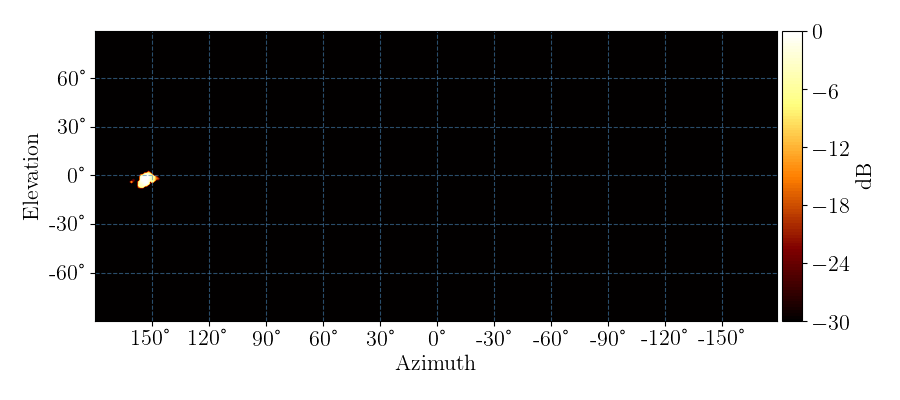
\includegraphics[width=0.8\textwidth]{Figures/chalkHi300MinPow.png}
\end{subfigure}
\vskip \baselineskip
\begin{subfigure}[b]{0.96\textwidth}
    \centering
    \includegraphics[width=0.8\textwidth]{Figures/chalklow300MinPow.png}
\end{subfigure}
\vskip \baselineskip
\begin{subfigure}[b]{0.96\textwidth}
    \centering
    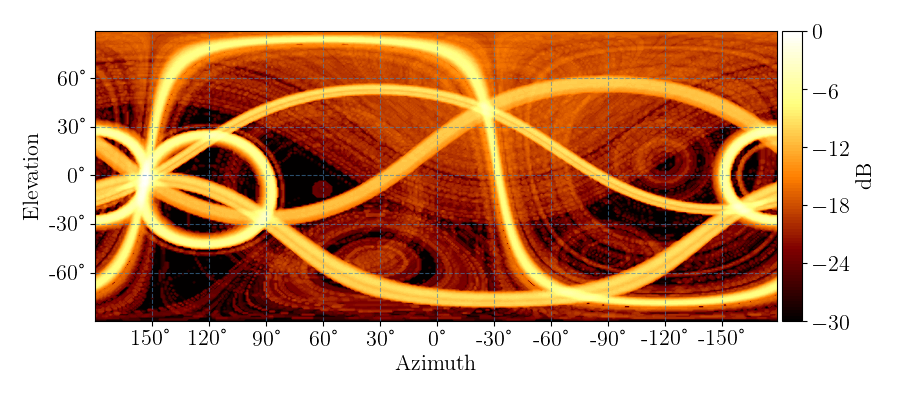
\includegraphics[width=0.8\textwidth]{Figures/chalkHi300Normal.png}
\end{subfigure}
\vskip \baselineskip
\begin{subfigure}[b]{0.96\textwidth}
    \centering
    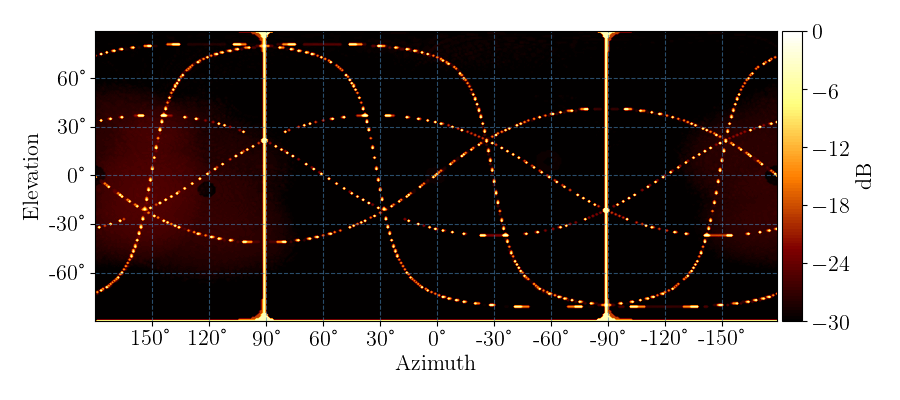
\includegraphics[width=0.8\textwidth]{Figures/chalkLow300Normal.png}
\end{subfigure}
\caption{Figures depict from top-to-bottom level SRP-PHAT localization results with high pass and low pass at 300Hz}
\label{fig:hilowfilter}
\end{figure}